\documentclass[12pt,letterpaper]{article}

\PassOptionsToPackage{hyphens}{url}
\usepackage[pdftex, bookmarksopen=true, bookmarksnumbered=true,
pdfstartview=FitH, breaklinks=true, urlbordercolor={0 1 0}, citebordercolor={0 0 1}]{hyperref}

% === MARGINS ===
\addtolength{\hoffset}{-0.75in} \addtolength{\voffset}{-1.25in}
\addtolength{\textwidth}{1.5in} \addtolength{\textheight}{2.25in}

% == ENVS ==
\newenvironment{tightcenter}{%
  \setlength\topsep{0pt}
  \setlength\parskip{0pt}
  \begin{center}
}{
  \end{center}
}

% == PACKS ==
\usepackage{color,soul}
\usepackage{graphicx}
\usepackage{calc} % To scale \pagewidth with \real{float}
\usepackage{pgfplots} % To draw histogram
\pgfplotsset{compat=1.17} % request specific version of pgfplots
\usepackage{calc} % to use \real for text -> numeric
\usepackage{pgf} % to store numeric variables
\usepackage{subcaption} % to place two figures horizontally
\usepackage{tikz}
\usetikzlibrary{automata,positioning}
\usetikzlibrary{arrows.meta, positioning, automata}
\tikzset{
  font={\fontsize{10pt}{0}\selectfont}}
\usepackage{forest}
\tikzset{
  Decision/.style = {%
    draw,
    line width=1.4pt
  },
  Lottery/.style = {%
    draw,
    line width=1.4pt
  },
  Outcome/.style = {%
    circle,
    minimum width=3pt,
    fill,
    inner sep=0pt
  }
}


  % == BIBS ==
\usepackage{natbib}
\bibliographystyle{apsr}

% == SPACES == 

% == CMMDS ==
\newcommand{\tit}{
\bf 
Finding General Citation Pattern in Internation Legal System using Text Information
}
\newcommand\spacingset[1]{\renewcommand{\baselinestretch}
{#1}\small\normalsize}

% == VARS == 
\pgfmathsetmacro{\heatmap}{1}

% == START (PageCounter, Mode)
\begin{document}

\spacingset{1.25}

\setcounter{page}{0}
\vspace{-.1in}

% == TITLE (includes DraftDate)
{\title{
    \tit
    % \thanks{Thanks to everyone in KimResearch Group}
  }
  \author{Suyeol Yun
    % \thanks{Applicant. No Affiliates. Email: \href{mailto:syyun@snu.ac.kr}{syyun@snu.ac.kr}}}
    % \date{First Draft: October 2, 2020\\ This Draft: \today
  }
  \maketitle
}

\thispagestyle{empty}
\vspace{-.1in}

\begin{abstract}

  % Legal citation pattern in the World Trad Organization (WTO) is quite complex to understand.
  % Legal citation pattern made by the member states of the World Trade Organization (WTO) shows how members of the WTO are understanding the legal system of the WTO,
  % it is is important to recover this complex pattern efficiently. To address this issue, this paper introduces a new method
  % to map this citation pattern as a network of articles of the WTO agreement.
  % First, this paper shows why we need to use the text information in the content of the trade dispute and legal text to successfully recover the citation pattern. 
  % Then this research designs a deep neural network model to extract information inside the text content.
  % After that, we are engaging machine learning algorithm to extract the citation pattern lying in the citation pattern predicted by the neural network. By doing so, this paper introduces clusters that are found by this method that are well capturing the most important principle in the World Trade Organization.

\end{abstract}

\spacingset{1.5} % gives a slightly more margin between abstract and introduction

\section{Introduction}

Inter-country interactions in global trade are legally regulated by the World Trade Organization (WTO).
The members of the WTO agreed on the set of rules with the WTO agreement and sue other country's potential
violation of the rules to the Dispute Settlement Body (DSB) of the WTO.
When a country is suing other country to the DSB, they usually cites more than one rules of the WTO
because a country's trade policy at issue is usually very complex thus requires many rules being combined to legallly blame the one successfully.
For example, In the Case A, Country X cited {Articles} to blame Country Y's TRADEACTION B.

Then why do political sceintist want to understand this complex pattern of citation? This is because of the two reasons,

- Finding the collective understanding over the WTO's system

- Second, upon/toward this understanding, countries design the new strategy to lead more favored result using the WTO.

However, the methods how to deal with this complexity, has been relatively less visited by the scholars. To address this issue, I designed
a new method that maps the countries' citation network over the WTO adjudication system. This method finds three distinctive clusters where each represents

- market access

- non-traiff barriers

- regional trade agreement
.

This method populates a network that can showing how countries are citing which articles together in which weight to legally regulate the trade disputes inside the WTO.
I explitly used the content of the dispute and the articles of the WTO agreement using deep neural network and machine learning algorithms.

Moreover, to populate this network, I used 80 GATT 1994 Articles or Paragraph in the Article with 143 Trade Disputes from 1995 to 2018 where the Panel reports exists.

Through this paper I found how wto works.
Moreover, this complexity efficietnly caputred by this mthod could address the legal capcity problem in the WTO.

\section{Data}
Privide a running example that explains how to works. (Borrow from previous paper)

\section{Methodology}
Example that simple approach can't aproach. (Limitation of co-occurrences)

\section{Empirical Findings}
No Greeks. English. Three Networks.

\section{Conclusion}
I show how WTO works.


\section{Appendix}
% == HEATMAP MATRIX == 
\begin{figure}[!tbp]
  \begin{subfigure}[b]{0.49\textwidth}
    \centering{
      \resizebox{\textwidth*\real{\heatmap}}{\textwidth*\real{\heatmap} * \real{1.7889}}{% This file was created by tikzplotlib v0.9.4.
\begin{tikzpicture}

\begin{axis}[
hide x axis,
hide y axis,
tick align=outside,
tick pos=left,
x grid style={white!69.0196078431373!black},
xmin=0, xmax=80,
xtick style={color=black},
y grid style={white!69.0196078431373!black},
ymin=0, ymax=143,
ytick style={color=black}
]
\addplot graphics [includegraphics cmd=\pgfimage,xmin=0, xmax=80, ymin=0, ymax=143] {co-citation-004.png};
\end{axis}

\end{tikzpicture}
}
      \caption{Co-citation Matrix}
    }
    \label{fig:f1}
  \end{subfigure}
  \hfill
  \begin{subfigure}[b]{0.49\textwidth}
    \centering{
      \resizebox{\textwidth*\real{\heatmap}}{\textwidth*\real{\heatmap} * \real{1.7889}}{% This file was created by tikzplotlib v0.9.4.
\begin{tikzpicture}

\begin{axis}[
hide x axis,
hide y axis,
tick align=outside,
tick pos=left,
x grid style={white!69.0196078431373!black},
xmin=0, xmax=80,
xtick style={color=black},
y grid style={white!69.0196078431373!black},
ymin=0, ymax=143,
ytick style={color=black}
]
\addplot graphics [includegraphics cmd=\pgfimage,xmin=0, xmax=80, ymin=0, ymax=143] {pred_only.png};
\end{axis}

\end{tikzpicture}
}
      \caption{Prediction Matrix}
    }
    \label{fig:f2}
  \end{subfigure}
  \caption{\bf Spare \& Dense Representation}
\end{figure}

% == THREE SUBSYSTEM == 
\begin{figure}
  \centering{
    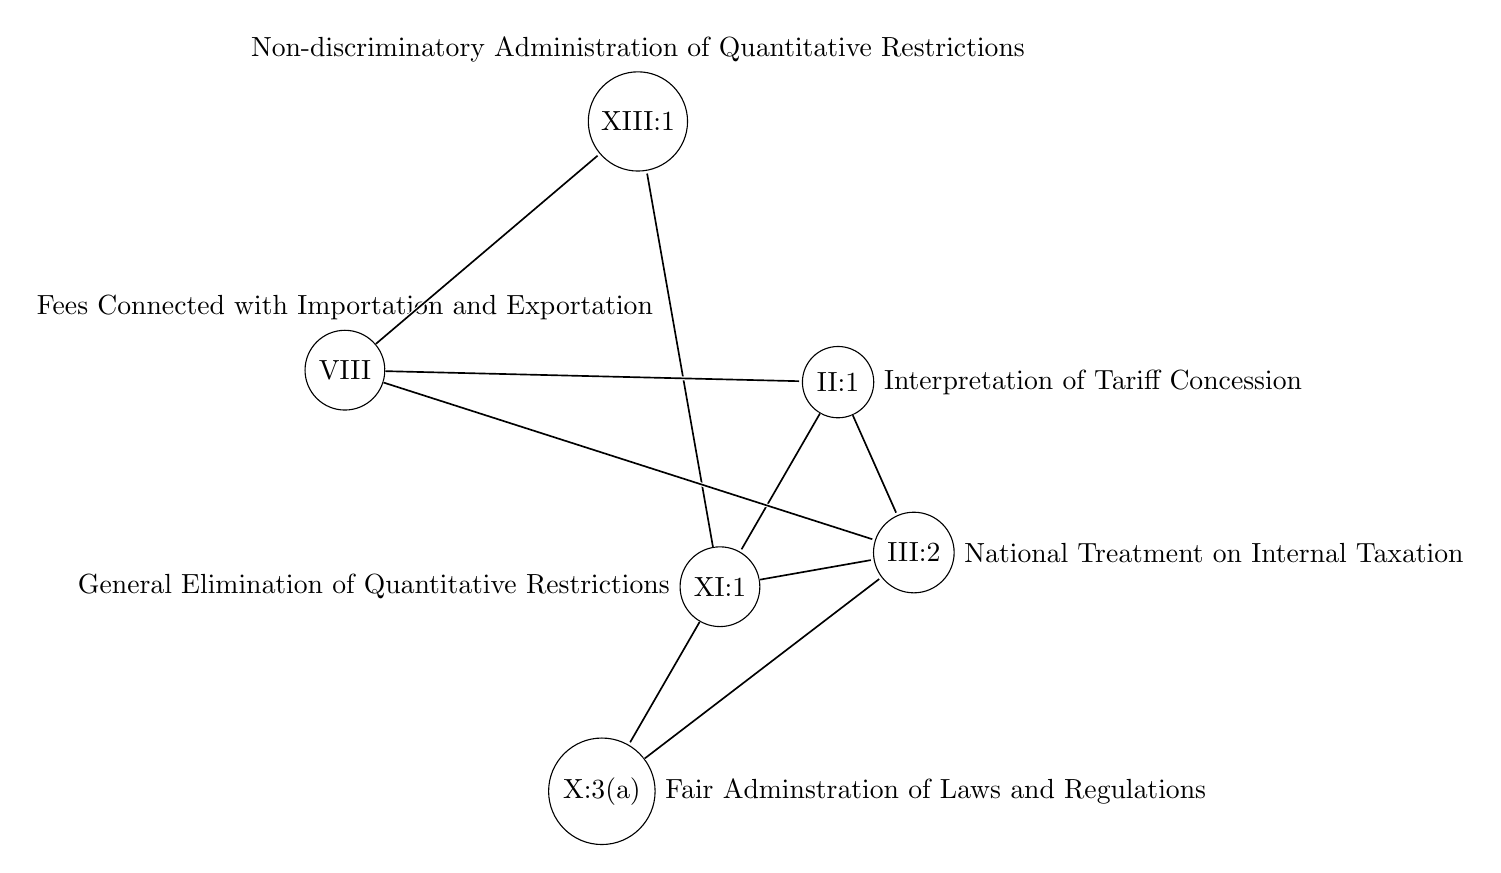
\begin{tikzpicture}[>={Stealth[color=black]},shorten >=1pt,node distance=2cm,on grid,initial/.style={}]
  \node[state, label=right:Interpretation of Tariff Concession] (T1) {II:1};
  \node[state, label=left:General Elimination of Quantitative Restrictions] at ([shift=({240:3 cm})]T1) (T4) {XI:1};
  \node[state, label=right:Fair Adminstration of Laws and Regulations] at ([shift=({240:3 cm})]T4) (T5) {X:3(a)};
  \node[state, label=above:Non-discriminatory Administration of Quantitative Restrictions] at ([shift=({100:6 cm})]T4) (T7) {XIII:1};
  \node[state, label=right:National Treatment on Internal Taxation] at ([shift=({10:2.5 cm})]T4) (T6) {III:2};
  \node[state, label=above:Fees Connected with Importation and Exportation] at ([shift=({150:5.5 cm})]T4) (T8) {VIII};

  \begin{scope}[every edge/.append style={-, double=black, draw=white}] % for directed edge, change "style={->, double=black, draw=white}]"
    \path (T1)
    edge   (T4)
    edge   (T6);
    \path (T4)
    edge   (T5)
    edge   (T6)
    edge   (T7);
    \path (T5)
    edge   (T6);
    \path (T8)
    edge   (T7)
    edge   (T1)
    edge   (T6);

  \end{scope}
\end{tikzpicture}

% to draw the node's border w/ color, refer to https://tex.stackexchange.com/questions/438412/how-to-add-border-to-a-node
  }
  \caption{Market Access}
  \label{fig:f2}
\end{figure}


% == END
\end{document}